%for a more compact document, add the option openany to avoid
%starting all chapters on odd numbered pages
\documentclass[12pt]{cmuthesis}

% This is a template for a CMU thesis.  It is 18 pages without any content :-)
% The source for this is pulled from a variety of sources and people.
% Here's a partial list of people who may or may have not contributed:
%
%        bnoble   = Brian Noble
%        caruana  = Rich Caruana
%        colohan  = Chris Colohan
%        comar    = Cyrus Omar
%        jab      = Justin Boyan
%        josullvn = Joseph O'Sullivan
%        jrs      = Jonathan Shewchuk
%        kosak    = Corey Kosak
%        mjz      = Matt Zekauskas (mattz@cs)
%        pdinda   = Peter Dinda
%        pfr      = Patrick Riley
%        dkoes = David Koes (me)

% My main contribution is putting everything into a single class files and small
% template since I prefer this to some complicated sprawling directory tree with
% makefiles.

% some useful packages
\usepackage{times}
\usepackage{fullpage}
\usepackage{graphicx}
\usepackage{amsmath}
\usepackage[numbers,sort]{natbib}
\usepackage[backref,pageanchor=true,plainpages=false, pdfpagelabels, bookmarks,bookmarksnumbered,
%pdfborder=0 0 0,  %removes outlines around hyper links in online display
]{hyperref}
\usepackage{subcaption}

\usepackage[capitalize,noabbrev,nameinlink]{cleveref}
\usepackage{float}
\usepackage[scaled]{inconsolata}

\captionsetup{labelfont=bf}
% \captionsetup{font=small}
\captionsetup{labelfont=bf}
\captionsetup{textfont={}}
%\captionsetup[subfloat]{font=small}
%\captionsetup[subfloat]{farskip=5pt}
%\captionsetup[subfloat]{captionskip=1pt}

\newcommand{\dbSQL}[1]{\texttt{\textbf{#1}}\xspace}

\DeclareUnicodeCharacter{0097}{~}


% Approximately 1" margins, more space on binding side
%\usepackage[letterpaper,twoside,vscale=.8,hscale=.75,nomarginpar]{geometry}
%for general printing (not binding)
\usepackage[letterpaper,twoside,vscale=.8,hscale=.75,nomarginpar,hmarginratio=1:1]{geometry}

% Provides a draft mark at the top of the document. 
\draftstamp{\today}{DRAFT}

\begin {document} 
\frontmatter

%initialize page style, so contents come out right (see bot) -mjz
\pagestyle{empty}

\title{ %% {\it \huge Thesis Proposal}\\
{\bf Code Generation Log Replay for In-memory Database Management Systems}}
\author{Tianlei Pan}
\date{June}
\Year{2021}
\trnumber{}

\committee{
Andy Pavlo, Chair \\
Wenting Ye \\
}

\support{}
\disclaimer{}

% copyright notice generated automatically from Year and author.
% permission added if \permission{} given.

\keywords{Code Generation, Log Replay, Recovery, Query Compilation}

\maketitle

\begin{dedication}
\end{dedication}

\pagestyle{plain} % for toc, was empty

%% Obviously, it's probably a good idea to break the various sections of your thesis
%% into different files and input them into this file...

\begin{abstract}
Instead of interpreting log records, we are extending our query code generation engine to create custom programs to replay log records. We will also be exploring for different optimization techniques to improve the recovery speed of recovery with code generation.
\end{abstract}

\begin{acknowledgments}
yes
\end{acknowledgments}



\tableofcontents
\listoffigures
\listoftables

\mainmatter

%% Double space document for easy review:
%\renewcommand{\baselinestretch}{1.66}\normalsize

% The other requirements Catherine has:
%
%  - avoid large margins.  She wants the thesis to use fewer pages, 
%    especially if it requires colour printing.
%
%  - The thesis should be formatted for double-sided printing.  This
%    means that all chapters, acknowledgements, table of contents, etc.
%    should start on odd numbered (right facing) pages.
%
%  - You need to use the department standard tech report title page.  I
%    have tried to ensure that the title page here conforms to this
%    standard.
%
%  - Use a nice serif font, such as Times Roman.  Sans serif looks bad.
%
% Other than that, just make it look good...


\chapter{Introduction}
A \textit{database management system (DBMS)} is a software that is responsible for storing data, analyzing data, and interacting with applications. Depending on the use case, a DBMS can be designed to focus more on either capturing data, or analyzing data. \textit{On-line Analytical Processing (OLAP)} applications focus on reading, analyzing and aggregating cold data that is less likely to be modified. On the other hand, \textit{On-line Transaction Processing (OLTP)} applications work with write-heavy transactions that modify the database frequently.

Consequently, recovery and durability in OLTP applications are more of a pressing issue compared to OLAP systems. Naive or manual backups are usually sufficient for read-only OLAP applications. However, since OLTP databases are being updated by transactions constantly, naive backups will either cause the database to lose significant amount of data, or fail to preserve the \textit{ACID (atomicity, consistency, isolation, and durability)} properties. This requires OLTP applications to develop specialized recovery mechanism to handle these problems. Commercial DBMS often combines Write-ahead Logging (WAL) with checkpoints to preserve database durability.

In addition, OLTP systems also require specialized algorithms and implementations to execute write transactions. Query compilation is an important optimization technique used in OLTP systems to greatly reduce the number of instructions that need to be executed. A DBMS uses a processing model (e.g. Iterator, Vectorization, Materialization) to determine how the DBMS executes a query plan. The processing model is responsible for translating a query into an intermediate expression. The execution engine then breaks down the expression into various tasks for execution. To speed up this process, the DBMS can use an optimization technique known as \textit{Query Compilation}. Query compilation requires the DBMS to generate specialized code for execution tasks to increase execution throughput. These specialized code are often created using an off-shelf compiler into a C/C++ program that implements the functionality of a certain query.

While query compilation has proved successful in increasing the efficiency of a DBMS, it comes with several drawbacks. Implementing a query compilation system can be quite an ordeal. It requires additional knowledge of compiler systems (e.g. LLVM) and huge amounts of engineering work to translate different execution tasks. Moreover, the DBMS also need to modify other components to accommodate with an execution engine reliant on query compilation.

One of such components is the recovery system. Since the execution engine has adapted to executing compiled native code, the DBMS needs to implement an additional execution engine to interpret the log records. Instead, we propose a system design that will extend the query execution engine to create custom programs for replaying log records.

\chapter{Background}
\section{Database Recovery}
\begin{figure}[H]
\centering
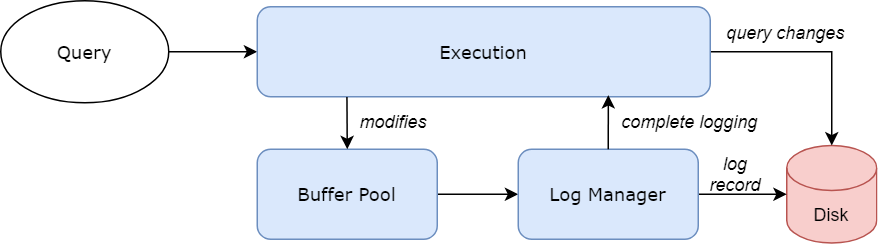
\includegraphics[width=0.9\textwidth]{images/Logging.png}
\caption{Write Ahead Logging.}
\label{fig:logging}
\end{figure}
Database recovery systems are responsible for preserving the ACID principles of a DBMS in case of failure. Prior to 1980s, early recovery systems rely heavily on non-volatile memory storage. Most of the DBMSs were disk-based and the recovery protocols assume the existence of dirty pages. System R\cite{system_r}, for instance, creates shadow copy of updated pages and maintains log record updates. Nowadays, both the capacity and reliability of main memory have increased significantly. This greatly improved the capabilities of in-memory DBMSs, but their performance is still be threatened by the need to synchronize non-volatile memory with persistent storage. Modern recovery systems aim to reduce the synchronization overhead.

Recovery systems consist of two components: logging and recovery. Logging is the action of storing transactional information on disk. These information are stored in a special data structure called a log record. A log record can either contain physical information (e.g. changes made to a specific physical address) or higher-level information (e.g. user-input query). In Write-ahead logging \cite{aries}, the DBMS records database changes in a log file before the changes can be persisted on disk. Each log record in the log file usually consists of redo records (install the effects of a committed transaction) and undo records (remove the effects on an incomplete or aborted transaction). Since in-memory DBMSs do not persist uncommitted changes, undo records are no longer required for the recovery system.

Recovery is the action of restoring the database system into a consistent state. If available, the DBMS first attempts to restore its previously recorded checkpoint. The database then initiates the log replay process to go through every log record stored since that checkpoint. SiloR\cite{silo_r} uses physical logging, checkpoints and an epoch-based recovery system. Transactions are assigned with different epochs and can only be persisted when their epochs are smaller then the current persistent epoch. VoltDB\cite{malviya14} uses a form of physiological logging that reduces transaction execution overhead. SAP HANA\cite{lee18}, however, uses a log-less approach through parallel table replication.

\section{Query Compilation / Code Generation}
When a query arrives, the DBMS parses the query into an expression tree. Eventually, the optimizer of the DBMS converts the expression tree into a physical plan tree. The physical plan represents how the query will be executed. It usually consists of operators that specify physical operations on the DBMS (e.g. inserting values into a certain memory location). For instance, \dbSQL{UPDATE x SET col1 = -col1 WHERE col1 BETWEEN 0 AND 100} can be represented by an update plan tree with a sequential plan as a child. The execution engine then uses the plan tree for execution.

The Iterator model\cite{volcano} is widely used in many disk-based DBMS (e.g. ORACLE RDBMS, MySQL, Microsft SQL Server) to interpret plan trees. The model "iterates" over each operator by implementing a \dbSQL{next()} function in each operator that returns the next tuples to be operated. The expressions inside the operators are evaluated using the provided tuples and generates output tuples. This approach suffers from frequent virtual function calls for in-memory DBMS. The Materialization model reduces this overhead by processing all the input tuples and emitting all the outputs at once ("materializing" the result as a single row or column). The Materialization model is suitable for OLTP DBMS since each OLTP query only accesses a small number of tuples at a time. However, since the Materialization results are stored in an in-memory buffer, the execution throughput is then bound by the size of the available memory space. While disk-based DBMSs are less concerned about the in-memory access since most of their operations are disk-based, this is especially critical for in-memory DBMSs.

Vectorization and Query Compilation are two state-of-the-art techniques employed for in-memory DBMSs to reduce memory overhead\cite{kersten18}. The Vectorization model is a variant of the Iterator model. Instead of emitting a single tuple at a time, the Vectorization model emits a batch of tuples at a time to amortize the cost of memory access. The functions that operate on these tuples are also specialized to be able to take in a batch of tuples at a time and more efficient compared to iterating over a single tuple at a time.

\begin{figure}[H]
\centering
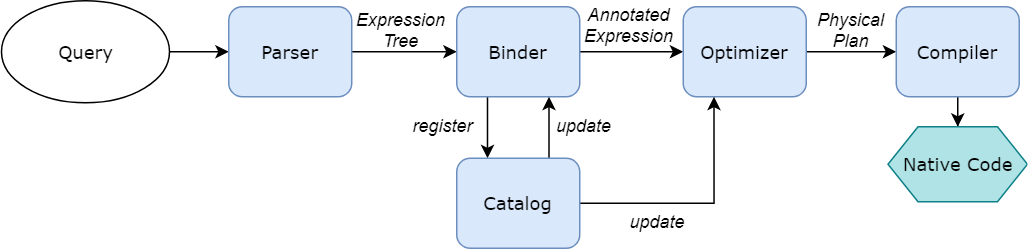
\includegraphics[width=0.9\textwidth]{images/QueryCompilation.png}
\caption{Query Compilation architecture.}
\label{fig:query_compilation}
\end{figure}

Query Compilation eliminates the cost of interpretation by compiling the physical plan to machine code. The machine code of the corresponding physical plan can then be executed repeatedly by the execution engine, removing any need for virtual function calls. Before being compiled to machine code, the physical plan is often first converted into an intermediate representation (e.g. C/C++ code, LLVM IR, or custom Domain Specific Language) that follows the grammar of an imperative language. This simplifies the process of converting the physical plan into machine code, as the intermediate representation form is designed to resembles closely to SQL statements. 

Hyper\cite{neumann11} is one of the pioneers of query compilation. It uses a data-centric compilation approach that splits the query plan into pipelines and compiles each pipeline separately. Vectorwise\cite{raducanu13} chooses to pre-compile huge amounts of micro function primitives that perform simple operations on typed data. During runtime, the DBMS can directly invoke these compiled primitives for query execution.

\chapter{Method}
\begin{figure}[H]
\centering
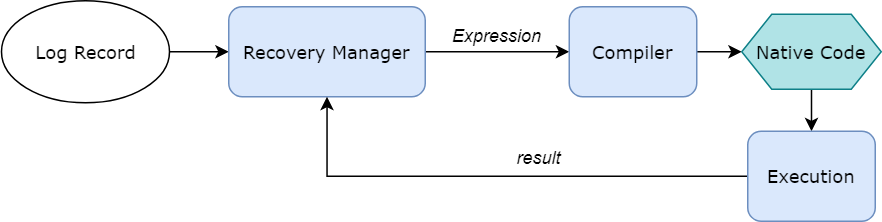
\includegraphics[width=0.9\textwidth]{images/Proposal.png}
\caption{Code Generation Recovery Mechanism.}
\label{fig:codegen_recovery}
\end{figure}

Our proposal is to extend the recovery layer and query compilation layer to support the interpretation of log records. This approach can be realized in three steps:

\begin{enumerate}
\item Extract information from log records.
\item Convert the information into expressions that can be accepted and compiled by the code generation engine (Code Generation Step).
\item Run the compiled machine code using the execution engine.
\end{enumerate}

This code generation approach brings around several benefits. Firstly, it significantly reduces engineering overhead. Compiling contents of the log records into machine code allows the recovery manager to seamlessly integrate with the built-in execution engine. This removes the need to specifically construct code to handle tasks that are not compiled to machine code.

\begin{figure}[H]
\centering
\begin{subfigure}{.5\textwidth}
 \centering
 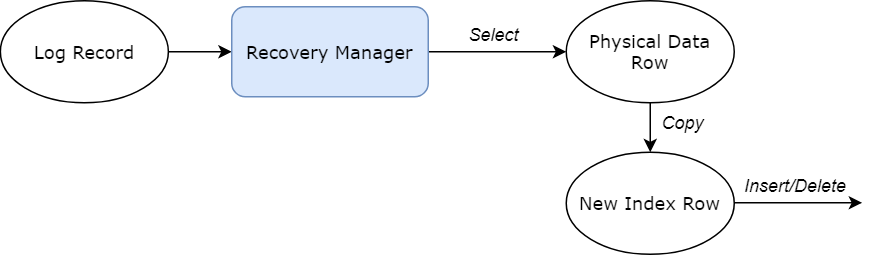
\includegraphics[width=0.9\textwidth]{images/RecoverIndex.png}
 \caption{Index Update During Recovery.}
  \label{fig:pipeline_graph}
\end{subfigure}%
\begin{subfigure}{.5\textwidth}
 \centering
 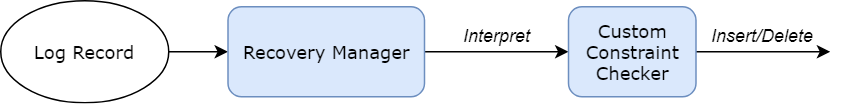
\includegraphics[width=0.9\textwidth]{images/RecoverConstraint.png}
 \caption{Constraint Checking During Recovery.}
  \label{fig:pipeline_code}
\end{subfigure}
\caption{Problems faced by conventional recovery in code generation DBMS.}
\label{fig:log_record}
\end{figure}

Secondly, it also resolves tricky problems that will appear when writing specialized code for log records. An example of this is index updates. Without code generation, the recovery manager needs to specifically reconstruct the index given an insert or update record. With code generation, the index updates are taken care directly by the execution engine that already contains high-performance specialized code for index maintenance. Similar problems, such as constraint checking

Our proposed architecture is implemented and tested in \textit{Noisepage} \cite{noisepage}, a self-driving in-memory DBMS developed at Carnegie Mellon University. Noisepage is built in C++ and uses the PostgreSQL wire protocol for user communication. The DBMS supports ACID transactions and \texttt{SNAPSHOT-ISOLATION}. Noisepage uses the conventional WAL recovery scheme with physical logging and depends on query compilation for query execution. We will dive into the details of Noisepage's recovery structure in the following sections.

\section{Recovery System Architecture}
\subsection{Transaction}
Transactions are the atomic operations of any DBMS. Noisepage uses a transaction to perform physical updates on the database and physical logging to disk. Noisepage uses a multi-versioned delta store transaction engine that ensures \texttt{SNAPSHOT-ISOLATION}. The transaction engine allows non-blocking reads over writes and vice versa, but does not allow write-write conflicts on a per tuple basis. A transaction's lifecycle begins when the transaction begins, and ends after the log manager has serialized its changes to disk.

Each data tuple in noisepage is uniquely identified through a tuple slot that stores the offset of a tuple. When the DBMS inserts a tuple into a table, it creates a new tuple slot that points to a memory location within the table. Subsequent updates to the tuple does not create direct copies of the tuple, but stores delta information (redo records) about the updates instead. These redo records are essential for executing log replay correctly. The structure of a redo record is shown later in \ref{fig:log_record}.

A transaction uses a buffer (redo buffer) that stores all the delta records that will appear in its lifetime. Each redo buffer has a fixed size of 4096 bytes and is allocated from a centralized buffer pool. Each time a transaction needs to change the contents of the DBMS, it will attempt to request space from the redo buffer to dump a corresponding delta record of the change. If the redo buffer runs out of space, the transaction will replace the current buffer with a new buffer from the buffer pool. The redo buffer allows the logging components to process the changes before the transaction is completed.

When a transaction commits, the transaction engine creates a commit record that contains a timestamp that refers to the oldest active transaction from the timestamp manager. The commit record is appended to the redo buffer. The redo buffer is then carried over to the log manager, where the changes will be serialized to disk. When a transaction aborts, the transaction creates an abort record that will prevent corresponding records to be replayed during recovery. Abort records are essential; since the redo buffer is persisted to disk by the log manager once it is full, it is possible for aborted transactions to persist on disk. Aborted transactions that are persisted on disk are rare, however, since it would be difficult for a typical OLTP transaction to fill up the entire redo buffer.

\subsection{Write-Ahead Logging}
\begin{figure}[H]
\centering
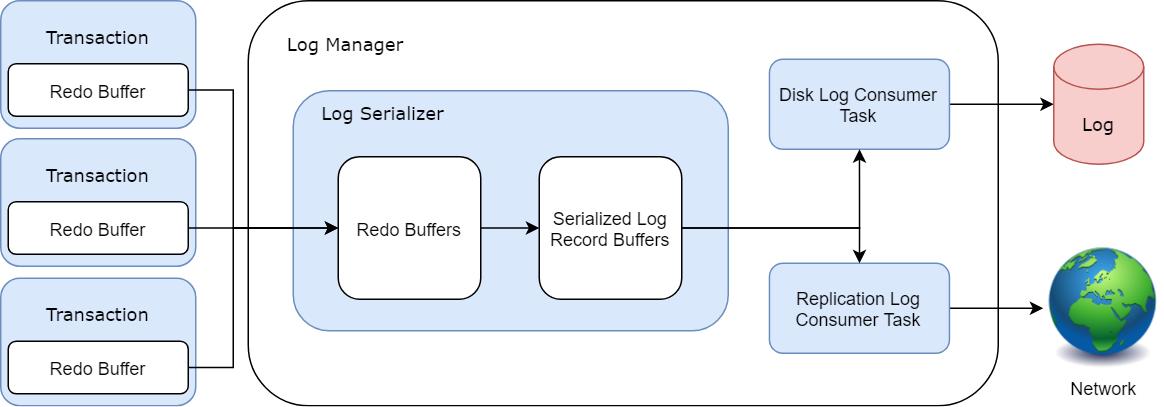
\includegraphics[width=0.9\textwidth]{images/WAL.png}
\caption{Logging Architecture. Log manager uses the log serializer and log consumers to convert redo buffers into log records.}
\label{fig:wal}
\end{figure}

The log manager is responsible for performing write-ahead logging in Noisepage. All the changes are serialized to disk as logs before they are performed on the DBMS storage. Each log record is self-contained and does not require any additional metadata to be replayed. The log manager consists of two separate tasks that live in different threads: the Log Serializer tasks and the Log Consumer tasks.

\subsubsection{Log Serializer}
The log serializer task receives redo buffers from a transaction once it is full, or when the transaction decides to commit. The log serializer breaks down the redo buffers into raw memory segmented into fixed-size buffers of 4096 bytes. These buffers will be consumed by the Disk Log Consumer for persistence.

The log records must be serialized in the correct order for recovery to perform correctly. Different transactions can share a same redo buffer that is filled with each of their own log records. Moreover, it is possible for transactions to appear in a non-serial order relative to their begin timestamp. However, the log records performed by an individual transaction is guaranteed to appear in the same order as they were created. This property helps ensure \texttt{SNAPSHOT-ISOLATION} property of Noisepage during log replay.
\subsubsection{Log Consumer}
Buffers supplied by the log serializer can be consumed by different log consumer tasks. Each log consumer is given a copy of the original buffer to achieve parallelism. Noisepage uses two type of log consumers: disk log consumer and replication log consumer.

The disk log consumer repeatedly polls for new buffers from the log serializer and writes the changes to disk. To improve performance, disk log consumer uses group commit that allows a batch of changes to be committed over a time period specified by the user. Under default settings, the disk log consumer writes down changes every 10 microseconds of if more than 1 MB of data has been written since the last write.

The replication log consumer also polls for new buffers, but instead of persisting them to disk, sends the new buffers over across the network to database replicas.

\subsection{Log Replay}
\begin{figure}[H]
\centering
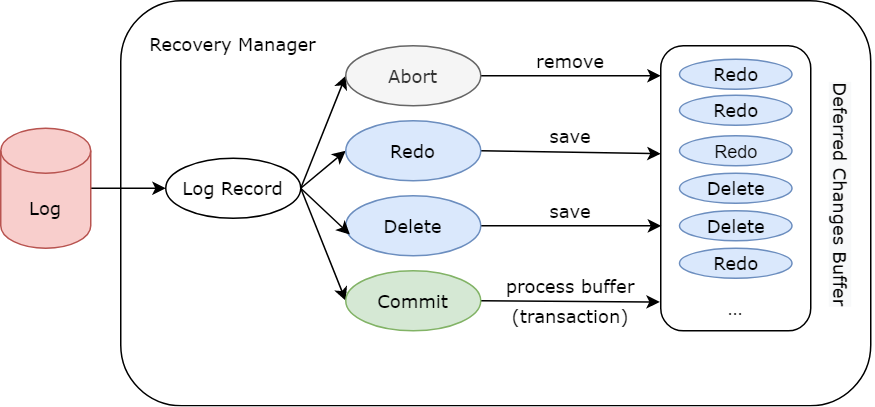
\includegraphics[width=0.9\textwidth]{images/RecoveryManager.png}
\caption{How recovery operates in Noisepage.}
\label{fig:recoverymanager}
\end{figure}

Noisepage uses four different record types: \textit{Redo, Delete, Commit, Abort}. Redo and Delete records are not processed immediately. Instead, they are placed inside a deferred changes buffer, ordered by their transaction timestamp. An Abort record removes the corresponding Redo/Delete record from the buffered changes. A Commit record initiates a transaction to iterate over the deferred changes buffer. Once all the deferred changes are processed, the buffer is cleared and the transaction is committed. The transaction aborts if any log record is malformed or any recovery operation fails.

\subsubsection{Data Structure}
\begin{figure}[H]
\centering
\begin{subfigure}{.5\textwidth}
 \centering
 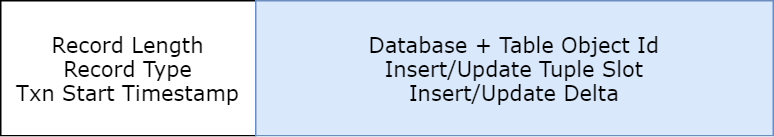
\includegraphics[width=0.9\textwidth]{images/RedoRecord.png}
 \caption{Redo Record Structure.}
  \label{fig:pipeline_graph}
\end{subfigure}%
\begin{subfigure}{.5\textwidth}
 \centering
 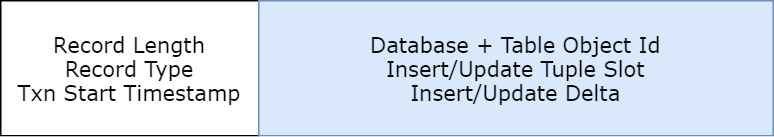
\includegraphics[width=0.9\textwidth]{images/DeleteRecord.png}
 \caption{Delete Record Structure.}
  \label{fig:pipeline_code}
\end{subfigure}
\caption{The internal log structures.}
\label{fig:log_record}
\end{figure}

A physical log record consists of a header followed by a record body. The header stores metadata about the log record itself, including its record type, size and begin timestamp of the transaction that generated the log record as mentioned in Section 3.1.1. The record body contains physical information that is necessary for recovery and varies depending on the record type. Depending on the value type, the values may bee stored in-line or not in-inline. Simple types such as \texttt{INTEGER}, \texttt{FLOAT} can be stored in-line, while \texttt{VARLEN} entry may stores the pointer in the values column that points to another location in the record.

Tuple slots in the log records will no longer be valid memory locations during recovery. Instead, the recovery manager creates an internal mapping from original tuple slots to a new tuple slots that will be retrieved after new values are inserted. The mapping allows the recovery manager to apply changes to the correct memory locations in the new memory environment.

Since only Redo and Delete records will effectively modify physical storage, we only need to analyze the record body of those two record types. Modifications of a query to the DBMS can be resolved down to the modification of tuple slots on the physical level.

\begin{figure}[H]
\centering
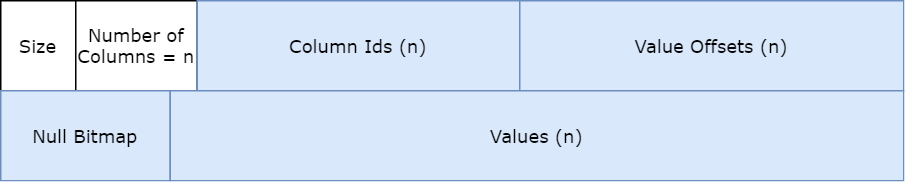
\includegraphics[width=0.9\textwidth]{images/Delta.png}
\caption{Redo Record Delta.}
\label{fig:logging}
\end{figure}

 While storing tuple slots is sufficient for delete records, Redo Records require additional data to perform Recovery Insert and Update operations. These data are kept in the Record Delta, which stores a mapping from column ids to values.

\subsubsection{Recovery Operation}
A Noisepage recovery step has three different operations:
\begin{itemize}
    \item \textbf{Insert}: Represented by a Redo Record. The recovery manager inserts the values stored within the redo record into the given tuple slot and updates the indexes.
    \item \textbf{Delete}: Represented by a Delete Record. The recovery manager deletes the tuple slot specified by the delete record and updates the indexes.
    \item \textbf{Update}: Represented by a Redo Record. The recovery manager updates the tuple slot using the values within the redo record and updates the indexes.
\end{itemize}

While both Insert and Update are represented using the same Redo Record structure, they can be differentiated by keeping track of all the tuple slots found in log records. If a tuple slot inside a Redo Record is unseen before, then the Redo Record represents an Insert operation. Otherwise, the Redo Record represents an Update operation.

\section{Recovery Code Generation}
The code generation structure in Noisepage follows from the data-centric compilation approach in \cite{neumann11}, as seen in \ref{fig:query_compilation}. A query is interpreted, optimized and converted into a physical plan tree. A plan tree consists of plan nodes and specifies how the query should be executed on the physical level of the database. 

A physical plan tree/node is then converted into an operator pipeline through a plan translator. Each plan translator correspond to a plan node in the original plan tree. A pipeline contains an ordered collection of relational operators that are not yet materialized, ended with a pipeline breaker (e.g. sort tuples, creating a hash table). The pipeline is only materialized whenever a pipeline breaker has been encountered.

\begin{figure}[H]
\centering
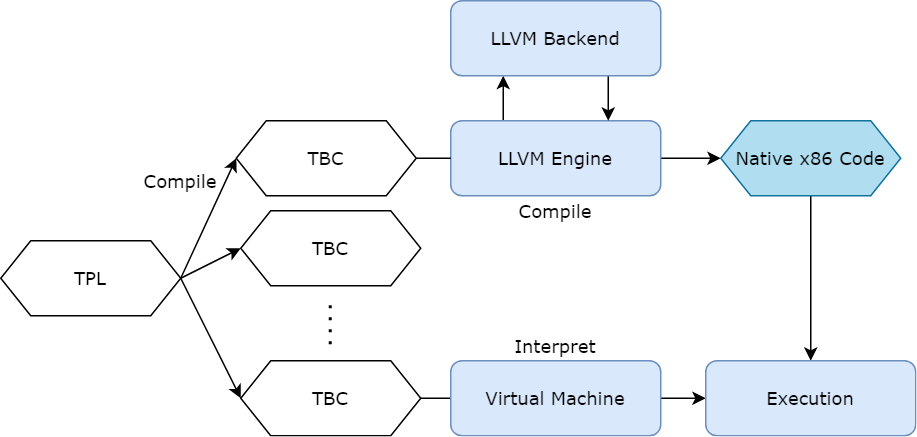
\includegraphics[width=0.9\textwidth]{images/LLVM.png}
\caption{Lifecycle of a TPL code fragment. Execution can run in either interpret or compile mode.}
\label{fig:llvm}
\end{figure}
Noisepage then compiles each operator pipeline into a domain-specific language referred to as TPL. Each function of a query inside the TPL code is then compiled to bytecode called TBC. TBC can be interpreted by a built-in virtual machine, or further compiled into an LLVM module. The execution engine can either interpret TBC, or run the compiled LLVM module.

\begin{figure}[H]
\centering
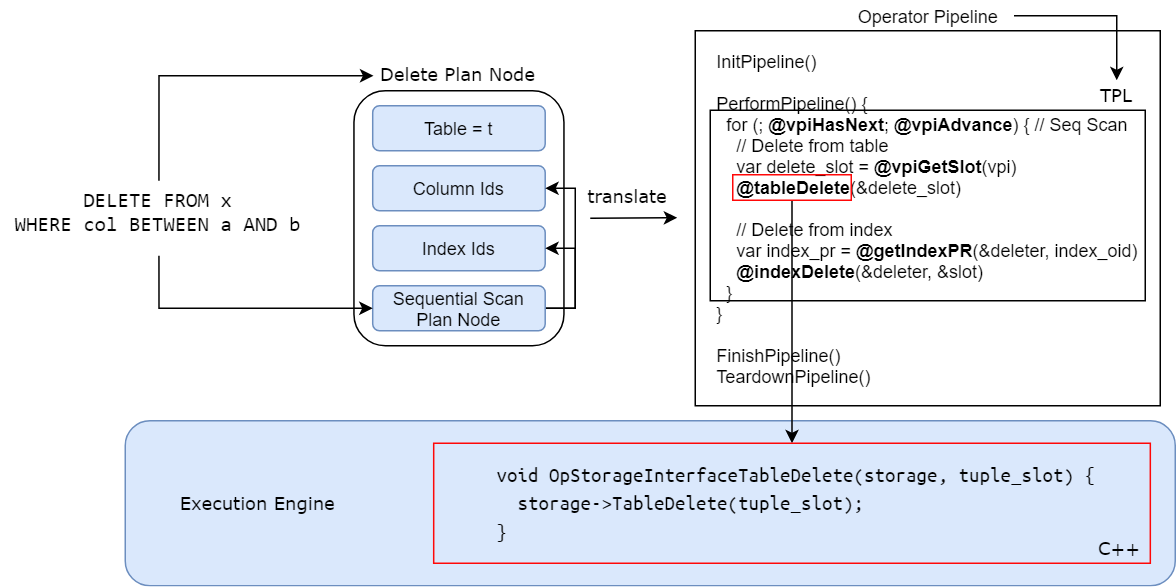
\includegraphics[width=0.9\textwidth]{images/CodegenExample.png}
\caption{Code Generation of \dbSQL{DELETE FROM x WHERE col BETWEEN a AND b}}
\label{fig:codegen_example}
\end{figure}

We further demonstrate the process of query compilation through the example in \ref{fig:codegen_example}. To run the query \dbSQL{DELETE FROM x WHERE col BETWEEN a AND b}, the DBMS needs to first do a sequential scan to find out the columns, and then do a delete operation on the found columns. These two steps are manifested in the delete plan node that includes a sequential scan plan node as a child. The plan node is translated into an operator pipeline that specifies how each operation will be exactly executed in the DBMS. The operator pipeline is then converted to TPL code. Each function inside the TPL code correspond to a piece of function inside the execution engine that will be evetually invoked once the compiled native code is run. For instance, \texttt{@tableDelete} corresponds to a C++ function \texttt{OpStorageInterfaceTableDelete} (a delete operation on a tuple slot of a table) in the execution engine.

\begin{figure}[H]
\centering
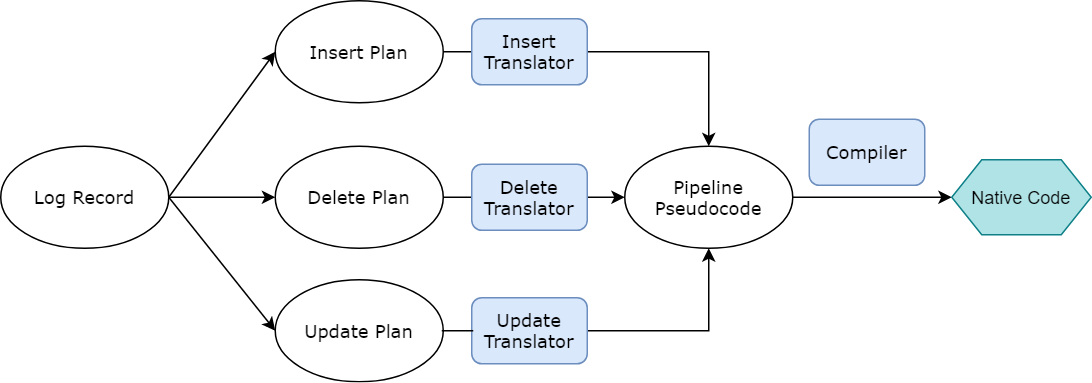
\includegraphics[width=0.9\textwidth]{images/ExpressionGeneration.png}
\caption{Process for converting log records into native code.}
\label{fig:logging}
\end{figure}
We imagine each recovery operation as a form of SQL statement that can be converted into native code through the code generation process discussed above. The code generation process for a log record can be divided into two steps: plan generation (creating the physical plan node) and plan translation (translating the plan into pipelines). Each recovery operation (\textbf{Insert}, \textbf{Update}, \textbf{Delete}) will be matched to a corresponding plan node.

\subsection{Insert Operation Conversion}

\begin{figure}[H]
\centering
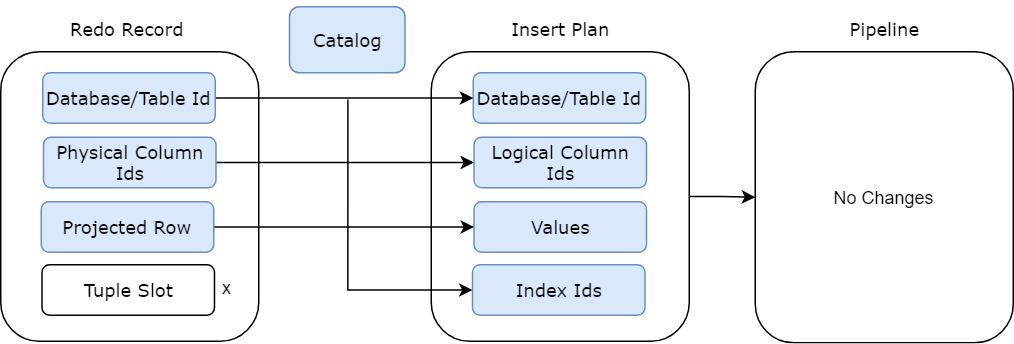
\includegraphics[width=0.9\textwidth]{images/InsertConversion.png}
\caption{Conversion from an Insert Redo Record into an Insert Plan Node. The tuple slot provided by the redo record is discarded.}
\label{fig:insert_conversion}
\end{figure}
Insert plan nodes correspond to \texttt{INSERT} statements. For an insert redo record, we can represent it as the SQL statement \dbSQL{INSERT INTO x VALUES y}. The insert plan node for this statement does not require a child plan node to function. This makes it straightforward to convert from an insert redo record to a plan node. Index information and column ids can be retrieved from the catalog. Values stored in the redo records are in their most basic form (e.g. integer, float, double) as constants and can be converted into expressions to be accepted by the insert plan node. The operation of transferring values, however, require one-to-one copy of each value from the log record into the plan node. 

\subsection{Delete Operation Conversion}
\begin{figure}[H]
\centering
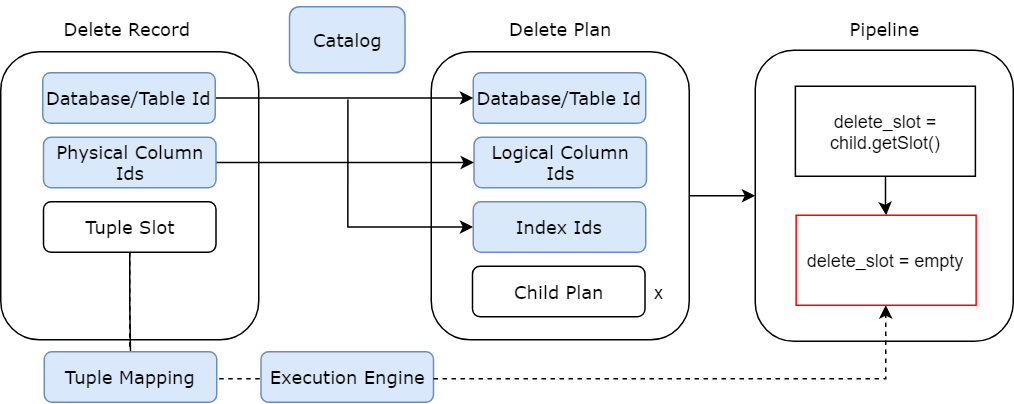
\includegraphics[width=0.9\textwidth]{images/DeleteConversion.png}
\caption{Conversion from a Delete Redo Record into a Delete Plan Node. Tuple slot that will be used in the pipeline is "smuggled" from the redo record through execution context.}
\label{fig:delete_conversion}
\end{figure}

Delete plan nodes correspond to \texttt{DELETE} statements and require child nodes to function. A delete plan node uses the child plan node to figure out which tuple slot to schedule for deletion. This is different for delete records. The mapping from recovery manager combined with the original tuple slot already points to the tuple slot to delete. In this case, there will be no need for the plan node to go through the child node and resolve the delete tuple slot. This is because, eventually, the delete plan node will attempt to create a Delete Record, which is structurally identical to the Delete Record from the recovery manager. Other operations, such as index deletions, are still necessary.

\subsection{Update Operation Conversion}
Update plan nodes correspond to \texttt{Update} statements and require child nodes to function. Unfortunately, update plan nodes are not very compatible with update redo records. After an update plan is translated into an update operator pipeline, it expects set clauses returned from the child node (e.g. sequential scan). These set clauses, however, describe higher-level logical operations and cannot be constructed easily as creating primitive expressions for insert plan nodes. 
\begin{figure}[H]
\centering
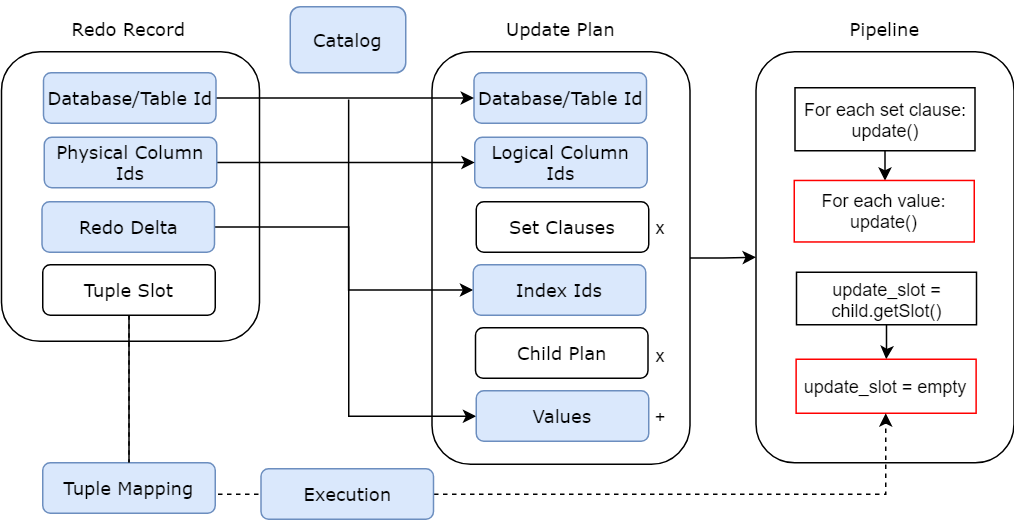
\includegraphics[width=0.9\textwidth]{images/UpdateConversion.png}
\caption{Conversion from an Update Redo Record into an Update Plan Node. Set clauses and child plan nodes inside the update plan node are discarded.}
\label{fig:update_conversion}
\end{figure}
The update plan node therefore needs to be extended to accept primitive values just like an insert plan node. We then modify the operator pipeline to process the primitive values instead of set clauses during a recovery step. Functions inside the operator pipeline will now apply to the primitive value expression. Similar to delete record transformations, there is no need for the update pipeline to resolve the update tuple slot or creating a new update record, as these information already exist in an update redo record and the tuple slot mapping in the recovery manager.


\section{Execution}
The compiled query is finally run by the execution engine. The compiled query invokes different operation codes (e.g. \texttt{OpStorageInterfaceTableDelete} in \ref{fig:codegen_example}) to complete the corresponding operator in the TPL code.


We explained earlier that the for physical plan nodes, they are expected to retrieve relevant tuple slots from the recovery manager, instead of supplying the tuple slots for an operation. We can circumvent this rule by modifying operation code functions.

\begin{figure}[H]
\centering
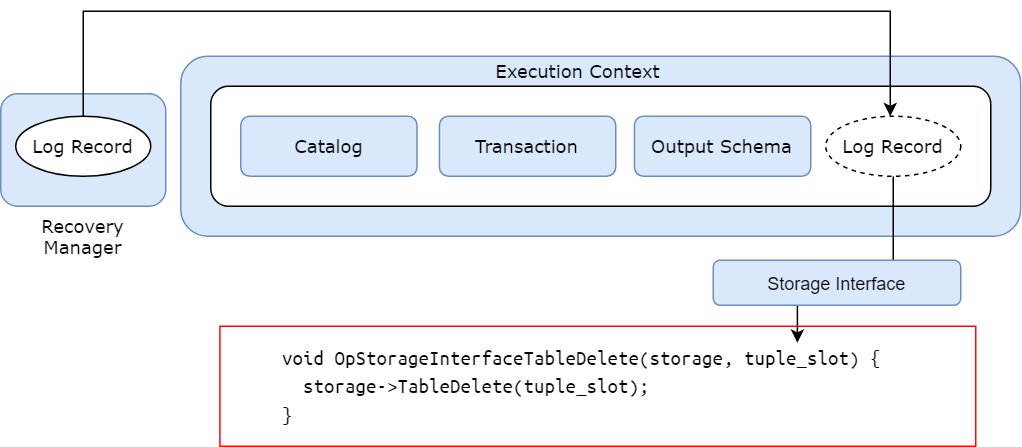
\includegraphics[width=0.9\textwidth]{images/RecoveryExecution.png}
\caption{Information from log record can be retrieved from the execution context.}
\label{fig:recovery_execution}
\end{figure}

An execution context encapsulates information that is supplied by upper layers of the DBMS. These information include access to the database catalog, the transaction running the query, etc. For our purposes, we can add tuple slot information into the execution context. Since the execution context can be accessed throughout the execution of a compiled query, we can modify the behavior of operation codes to override with the recovery tuple slots if necessary.

For Delete and Update operations, we need to supply the execution context with the log record itself. Since we modified the delete translator to skip the process of looking through child plan node for objects to delete, we will deliver the Delete Record from the recovery manager directly to the operation codes that will be expecting a Delete Record generated by a regular delete plan node.

\section{Caching Optimization}

The naive implementation for code generation searches for table metadata and re-compiles the native code every time the recovery manager reads in a new log record. This is very inefficient and requires huge amounts of memory access and copy. We can use caching techniques to reduce performance overhead.

\subsection{Metadata}
Most of the metadata overhead is generated during the conversion step from a redo record into an insert plan node. For each table, the DBMS needs to figure out its relevant metadata. These operations require frequent lookup into the database catalog. As long as those metadata are bound to some table id, the DBMS can cache those metadata and re-use them for the same table. Some significant metadata are listed below:

\subsubsection{Physical to Logical Column Mapping}
The recovery manager needs to maintain a mapping from physical column ids to logical column ids for each table. This is required because the column ids recorded in the log records are physical ids, while all the query compilation components expect logical column ids. The mappings can be generated by looking into the DBMS catalog.
\subsubsection{Column Value Type Mapping}
For redo records, the recovery manager also needs to maintain a mapping from each column to its corresponding SQL value type (e.g. \dbSQL{INTEGER, FLOAT, VARLEN}). This mapping is used to correctly copy the values out of each redo record into a physical plan node.

\subsection{Compiled Query}
A major benefit of Query Compilation is that the compiled query can be reused by the execution engine. If the contents of a physical plan node remains largely unchanged, then there is no need to reconstruct the physical plan every time the recovery manager processes a log record.

We can cache each type of recovery operation separately and use a combination of database and table id as unique identifiers. The cached query can be re-usesd as long as the table schema remains unchanged.

\subsubsection{Parameterization}
\begin{figure}[H]
\centering
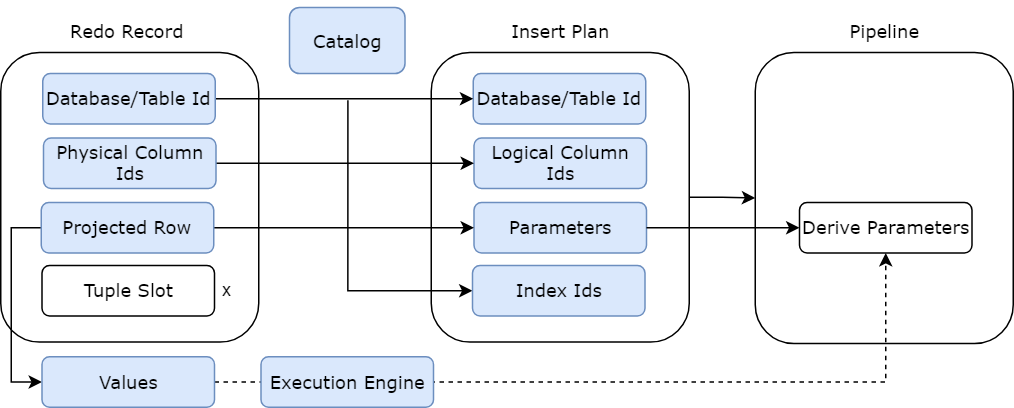
\includegraphics[width=0.9\textwidth]{images/ParameterizedRedoRecord.png}
\caption{Parameterized insert plan.}
\label{fig:parameterization}
\end{figure}

Caching is trickier for recovery operations that need to transfer values into plan nodes. A primitive expression will change every time its underlying value changes. A solution to this is to parameterize the primitive expression given to a insert/update plan node. During run-time, the execution context pass in actual values into the parameterized expressions. This approach allows a compiled query to keep value type information for each table column and remain flexible enough to swap in actual values without recompilation.

\chapter{Experimental Evaluation}
We run our experiments on Ubuntu 20.04.
Dual-socket 10-core Intel Xeon E5-2630v4 CPU, 128 GB of DRAM, and a 500 GB Samsung 970 EVO Plus SSD.

\section{Throughput Measurement}
\subsection{Insert}
We first measure the throughput (number of transactions executed per time period) of insert operations against the baseline recovery performance on a single table. The recovery manager uses only our insert implementation for recovery.
\begin{table}[H]
\begin{center}
\begin{tabular}{ |c|c|c| } 
 \hline
Statements Ratio & \textbf{Baseline Throughput} & \textbf{Codegen Throughput}\\ 
 \hline
 100\% Insert & $1.12 \times 10^4$ txns/s & $5.60 \times 10^3$ txns/s\\
 \hline
 50\% Insert, 50\% Select & $1.32 \times 10$ txns/s & $6.60 \times 10^3$ txns/s \\ 
 \hline
\end{tabular}
\caption{\textbf{Insert throughput measurement setup on a single table}. The table uses an initial table size of $10^6$. Each transaction runs 5 statements. A total of $10^5$ transactions are run.}
\label{tab:throughput_exp_insert}
\end{center}
\end{table}

2x difference. Memory copies.

\subsection{Delete}
We then measure throughput of delete operations against the baseline. The recovery manager uses only our delete implementation for recovery.
\begin{table}[H]
\begin{center}
\begin{tabular}{ |c|c|c| } 
 \hline
Statements Ratio & \textbf{Baseline Throughput} & \textbf{Codegen Throughput}\\
 \hline
 90\% Insert, 10\% Delete & $1.12 \times 10^4$ txns/s & $1.06 \times 10^4$ txns/s \\ 
 \hline
 80\% Insert, 20\% Delete & $1.11 \times 10^4$ txns/s & $1.07 \times 10^4$ txns/s\\
  \hline
 75\% Insert, 25\% Delete & $1.13 \times 10^4$ txns/s & $1.03 \times 10^4$ txns/s\\
 \hline
\end{tabular}
\caption{\textbf{Delete throughput measurement setup on a single table}. The table uses the same setup in \ref{tab:throughput_exp_insert}.}
\label{tab:throughput_exp_delete}
\end{center}
\end{table}

\subsection{Update}
Finally, we measure throughput of delete operations against the baseline. The recovery manager uses only our delete implementation for recovery.
\begin{table}[H]
\begin{center}
\begin{tabular}{ |c|c|c| } 
 \hline
Statements Ratio & \textbf{Baseline Throughput} & \textbf{Codegen Throughput}\\ 
 \hline
 90\% Insert, 10\% Update & $???$ txns/s & $???$ txns/s\\
  \hline
 75\% Insert, 25\% Update & $???$ txns/s & $5.6 \times 10^3$ txns/s\\
 \hline
 50\% Insert, 50\% Update & $???$ txns/s & $10^4$ txns/s \\ 
 \hline
\end{tabular}
\caption{\textbf{Update throughput measurement setup on a single table}. The table uses the same setup in \ref{tab:throughput_exp_insert}.}
\label{tab:throughput_exp_update}
\end{center}
\end{table}

\section{Throughput Measurement With Indexes}
In the baseline recovery architecture, the recovery manager implements a custom index update function that is independent from the query execution engine. This index update function is largely hard-coded and contains large amounts of memory copy operations. The code generation approach, however, use the built-in execution engine for index updates. We believe as the number of indexes increases, the performance gap between baseline and the code generation approach will shorten.
\begin{table}[H]
\begin{center}
\begin{tabular}{ |c|c|c|c|c| } 
 \hline
Statements Ratio & \#Indexes & \textbf{Baseline Throughput} & \textbf{Codegen Throughput} & \textbf{Baseline:Codegen} \\ 
 \hline
 100\% Insert & 5 & $3.7 \times 10^4$ txns/s & $2.4 \times 10^4$ txns/s & 1.54\\
 \hline
 100\% Insert & 10 & $2.4 \times 10^4$ txns/s & $1.7 \times 10^4$ txns/s & 1.41\\
 \hline
 100\% Insert & 100 & $3.2 \times 10^3$ txns/s & $2.4 \times 10^3$ txns/s & 1.3\\
 \hline
\end{tabular}
\caption{\textbf{Insert throughput measurement setup on a single table with indexes}. The table uses the same setup in \ref{tab:throughput_exp_insert}.}
\label{tab:throughput_exp_index_insert}
\end{center}
\end{table}

\section{Throughput Measurement With Constraints}

\chapter{Related Work}
\chapter{Conclusion}

%\appendix
%\include{appendix}

\backmatter

%\renewcommand{\baselinestretch}{1.0}\normalsize

% By default \bibsection is \chapter*, but we really want this to show
% up in the table of contents and pdf bookmarks.
\renewcommand{\bibsection}{\chapter{\bibname}}
%\renewcommand{\bibpreamble}{This text goes between the ``Bibliography''
%  header and the actual list of references}
\bibliographystyle{plainnat}
\bibliography{citations} %your bib file

\end{document}
